\documentclass[11pt,a4paper,DIV=9]{scrartcl}

\usepackage{pgf}
\usepackage{tikz}
\usetikzlibrary{arrows,automata,positioning,shadows}
\usepackage{ngerman}
\usepackage[utf8]{inputenc}
\usepackage{amsmath,amssymb}
\usetikzlibrary{shapes,snakes}
% Schriftart ändern
\renewcommand{\rmdefault}{ppl}
%Möglichkeit zur Änderung von Überschriften
\usepackage{sectsty}
%Überschrift \section uandern
\definecolor{blue}{RGB}{76 , 92, 153}
\allsectionsfont{\color{blue}}
\paragraphfont{\color{blue}}

%Variable Blattnummer
\newcommand{\blatt}[1]{
  \newcommand{\blattnr}{#1}
}
%Aufgabe und Aufgabenteil definieren
\newcounter{temp}
\newcommand{\aufgabe}[1]{
  \setcounter{temp}{\value{subsection}}
  \setcounter{subsection}{#1}
  \addtocounter{subsection}{-1}
  \subsection{Aufgabe}
  \setcounter{subsection}{\value{temp}}
}
\newcommand{\teil}[2][]{
  \subsubsection*{#2) #1}
}
\renewcommand{\author}[1]{\renewcommand{\author}{#1}}
\renewcommand{\title}[1]{\renewcommand{\title}{#1}}
\newcommand{\makehomeworktitle}{
  \begin{minipage}[t]{6.5cm}
    \sf{\author}
  \end{minipage}
  \begin{minipage}[t]{6.5cm}
    \begin{flushright}
      \sf{\title\\\today}
    \end{flushright}
  \end{minipage}
  \\[0.2cm]
  \begin{center}
    \sf{
      \color{blue}{
        \LARGE{Dokumentation \blattnr}
      }
    }
  \end{center}
  \vspace{0.1cm}
}

%%%%%%%%%%%%%%%%%%%%%%%%
%%% Statisch
\author{{[}4131658{]} Jan Germann \\{[}4054962{]} Christian Ratz\\Übungsgruppe 1}
\title{SQL Praktikum}

%%% Auf jedes Hausaufgabenblatt anpassen
\blatt{1}
%%%%%%%%%%%%%%%%%%%%%%%%
\begin{document}
\makehomeworktitle

\section{Einleitung}
  In dieser Dokumentation werden die Besonderheiten des Klassendiagramms, für das communitybasierte Musik-Streamingportal FIRST.FM, erläutert. Bei dem Musik-Streamingportal FIRST.FM, haben Benutzer die Möglichkeit selbstkomponierte Musik zu veröffentlichen, Musik anderer Benutzer oder Bands zu hören sowie selbst einer Band beizutreten.\\
  Am Ende dieser Dokumentation ist, zur besseren Übersicht, das komplette Klassendiagramm noch einmal in seiner Vollständigkeit zu finden.

  \subsection{Formatierung} 
    In der Dokumentation sowie im dazugehörigen Diagramm gilt die folgende Formatierung.

    \begin{description}
      \item [Klassennamen] \hfill \\
        Der Name einer Klasse ist \textbf{fett} formatiert.
      \item [Attribute] \hfill \\
        Attribute einer Klasse sind folgendermaßen gekennzeichnet
        \begin{itemize}
          \item[-] Reguläres Attribut
          \item[*] Attribut ist Teil des Primärschlüssel
          \item[/] Abgeleitetes Attribut
          \item[+] Fremdschlüssel
        \end{itemize}
      \item[Relationentypen] \hfill
      \begin{itemize}
        \item Reguläre Relationen zwischen Klassen sind durch eine einfache schwarze Linie gekennzeichnet.
        \item Sogenannte \textit{XOR}-Relationen besitzen an der ausgehenden Klasse ein Rautesymbol ($\blacklozenge$). Hierbei darf die Klasse, für gespeicherten Entität, nur mit einer einzigen der Klassen gleichzeit in Relation stehen.
      \end{itemize}
    \end{description}

\section{Klassen}
\subsection{}


\section{Klassendiagramm}
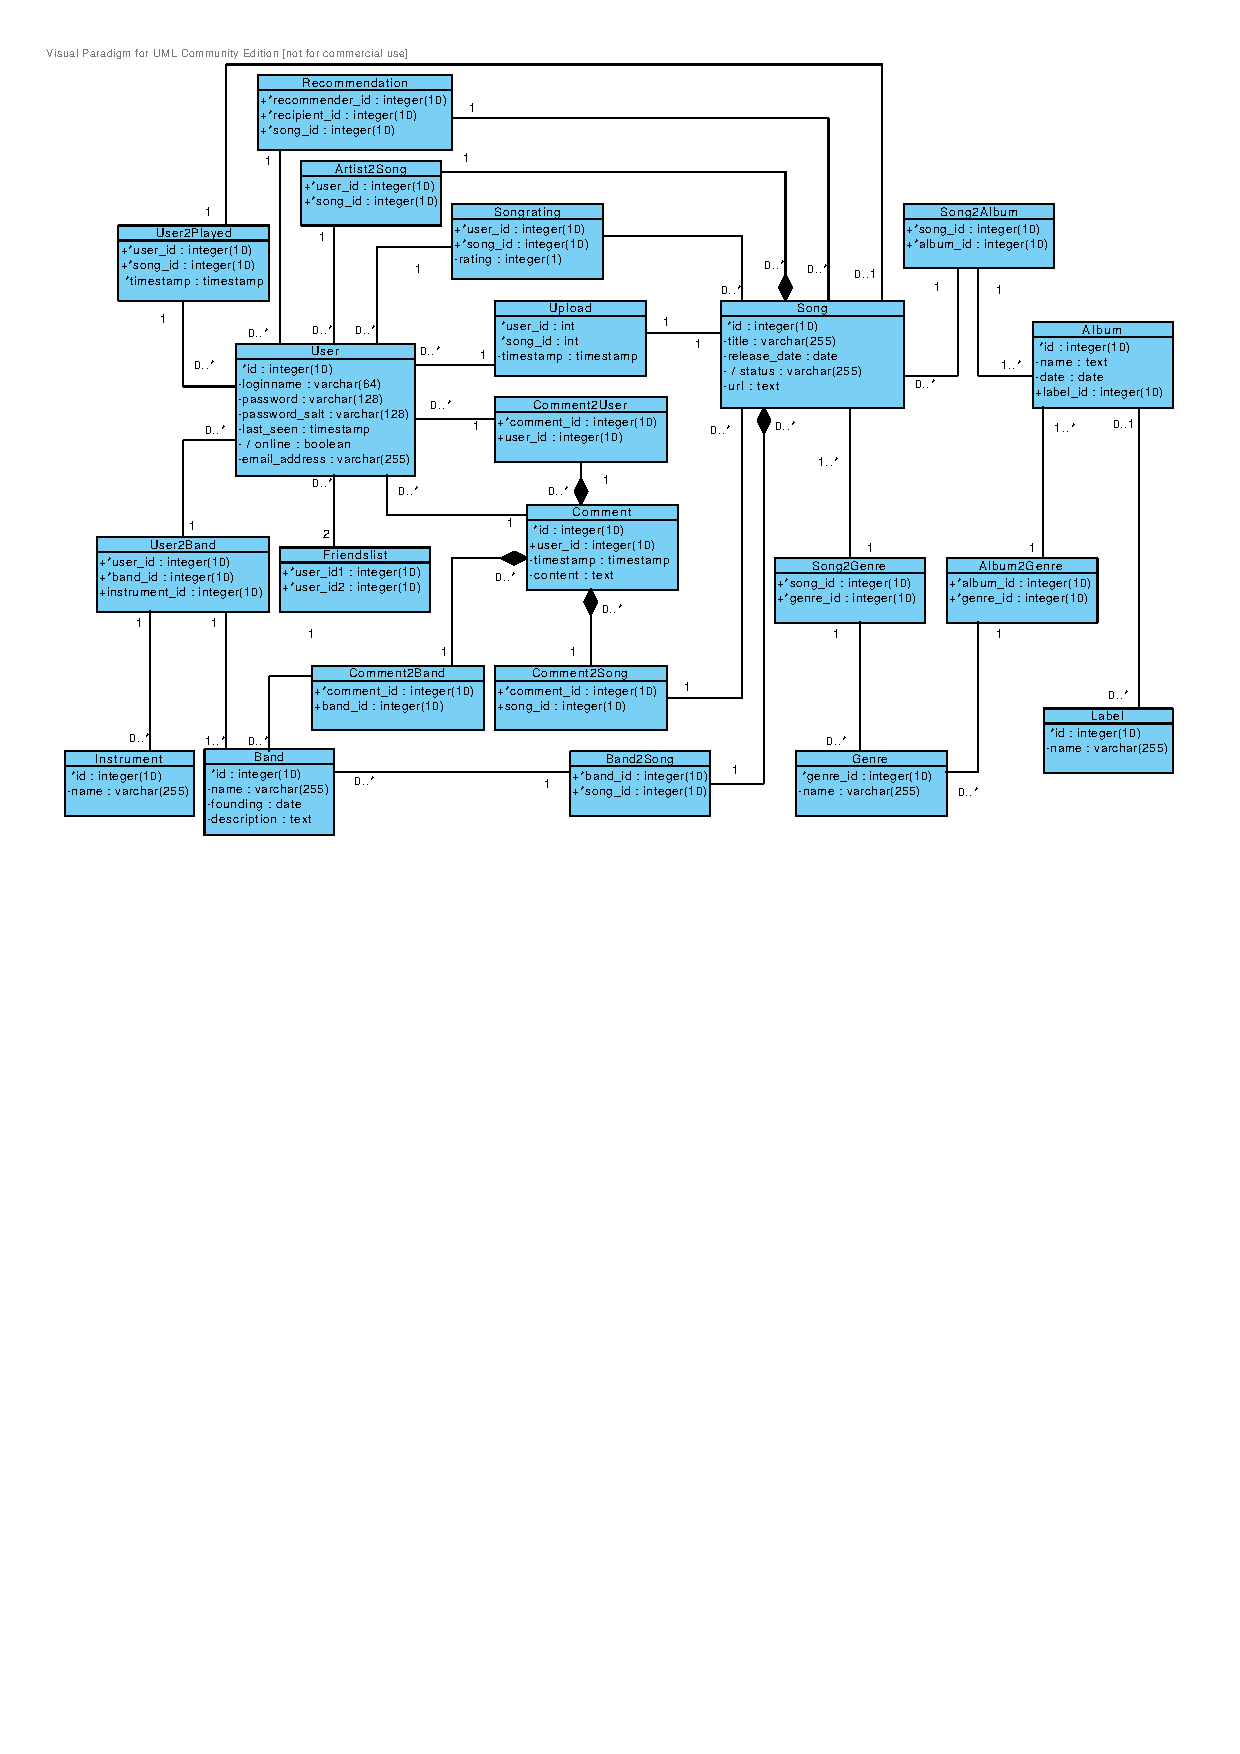
\includegraphics[page=1, angle=90,trim=0cm 0cm 0cm 1cm, clip=true]{Diagram1}
\end{document}